%!TEX root = pset1.tex

\section{Sparsity and LASSO}\label{sec:gen}
An alternative approach is to use the $L_1$ norm regularizer in the objective for regularized least squares.  The error function that we aim to minimize over is given by:
\begin{equation} \label{eq:lasso_error_fn}
\frac{1}{2} \sum_{n=1}^{N} (t_n - \M{w}^T \phi (\M{x}_n) )^2 + \frac{\lambda}{2} \sum_{j=1}^{M} |w_j|
\end{equation}

The LASSO is widely used in practice because it leads to solutions which are relatively sparse, i.e. the resulting prediction vector $\M{w}$ tends to have few non-zero components.  

To test this method and its sparsity properties, we consider a regression problem with 5 training points and 500 testing points in $\mathbb{R}^{12}$.  The data is generated according to  $f(x) = \M{w}^T \phi (\M{x}) + \epsilon$, where $\epsilon \sim  N(0,\sigma^2)$ and $\M{w} \in \mathbb{R}^{12}$ is a sparse vector with only two non-zero components.  For this problem, we assume that $\M{w}$ is unknown, and we estimate this vector with ridge regression in Section~\ref{sec:sparsity_ridge_reg} and with LASSO in Section~\ref{sec:sparsity_grad_desc}.  Let $\lambda_2$ denote the regularizer term for the $L_2$ norm and let $\lambda_1$ denote the regularizer term for the $L_1$ norm.  Figure~\ref{fig:lasso_sparsity} shows plots of the estimated function with different regularizers.  

\subsection{Ridge Regression Gradient Descent} \label{sec:sparsity_ridge_reg}
Applying our method for gradient descent to the ridge regression problem on the training dataset of 12 points, we compute the vector of weights $\M{w}$ and MSE on the testing dataset for $\lambda_2 = 0.1$.  We obtain: 
%
\begin{flalign*}
\M{w} &= (0.12,0.14,0.22,0.20,0.09,-0.05,-0.20,-0.30,-0.32,-0.25,-0.08,0.12)\\
\text{MSE} &=  0.2606.
\end{flalign*}
%
If we disable the $L_2$ regularizer (set $\lambda_2 = 0$), i.e., the OLS estimator, we obtain:
%
\begin{flalign*}
\M{w} &= (1.15,1.30,1.72,0.67,-1.73,-4.28,-5.16,-3.27,0.48,3.01,0.61,-8.83),\\
\text{MSE} &=  109.2910.
\end{flalign*}
%
\subsection{LASSO Gradient Descent} \label{sec:sparsity_grad_desc}
Similarly, we apply our method for gradient descent to the LASSO problem on the on the training dataset of 12 points.  For $\lambda_1 = 0.1$, we find: 
%
\begin{flalign*}
\M{w} &= (0.00,0.00,0.43,0.00,0.00,-0.00,-0.00,-0.00,-1.02,-0.00,-0.00,0.00),\\
\text{MSE} &=0.0487.
\end{flalign*}

\subsection{Sparsity Properties of LASSO}
We observe from Figure \ref{fig:lasso_sparsity} and MSE values that LASSO estimation is closest to the true value function, compared to ridge regression or non-regularized OLS. In terms of sparsity, LASSO estimator has only two variables that are non-zero (the rest are within numerically negligible deviation from 0), whereas the other estimators have non-sparse results. We believe that $l_0$ norm constraint (number of non-zero elements in $\V w$ less than $K$) is the true sparsity constraint; however, it is non-convex and difficult to solve directly, thus its convex hull-- the $l_1$ norm used in LASSO can be used as an approximation to often give sparse results. Even though $l_2$ norm regularization penalizes the size of $\V w$, it does not relate directly to the number of non-zero elements in $\V w$, and therefore does not provide sparse results.


\begin{figure}[h!]
\centering
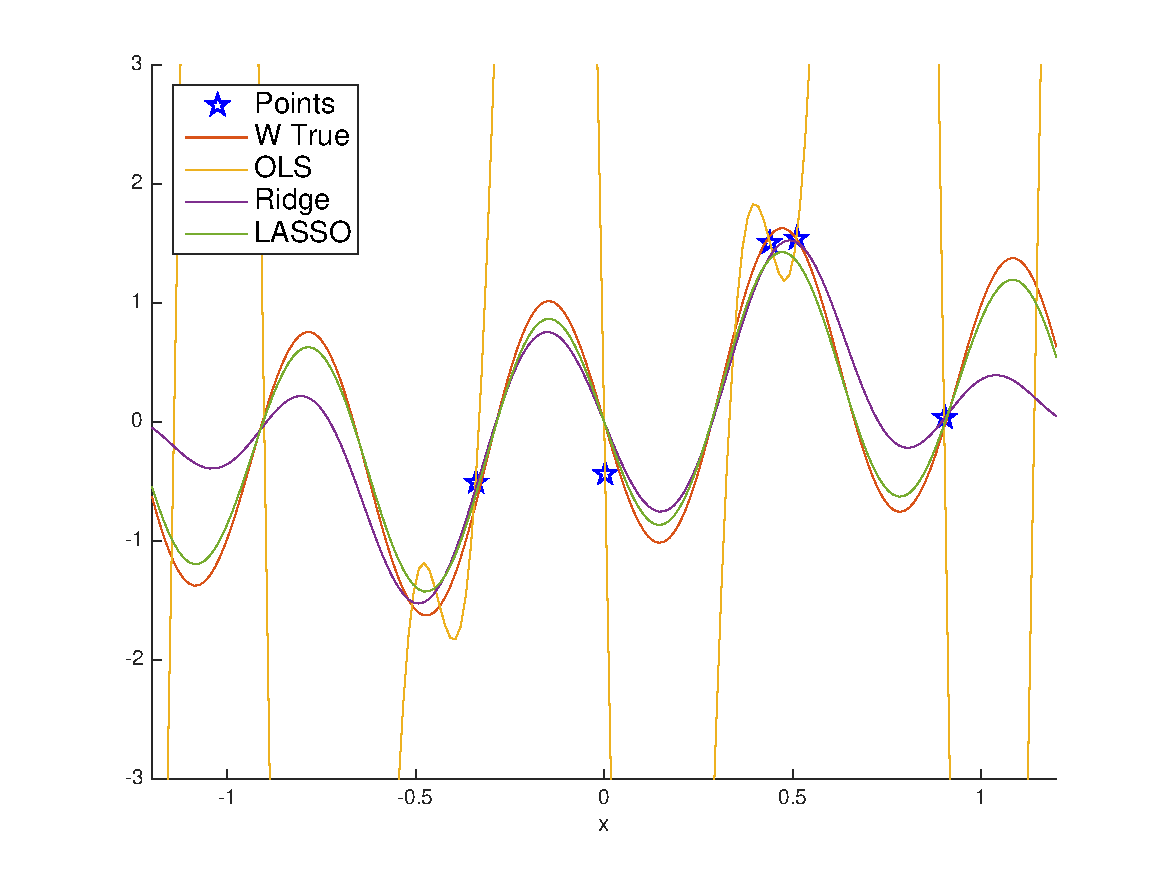
\includegraphics[scale=0.8]{hw1_4_1.pdf}
\caption{Plots of estimated function with different regularizers \\
OLS: $\lambda_1 = \lambda_2 = 0$, Ridge: $\lambda_2 = 0.1$, LASSO: $\lambda_1 = 0.1$.} \label{fig:lasso_sparsity}
\end{figure}